\documentclass[../../main.tex]{subfiles}


\begin{document}
\subsection*{(a)}
Import log-flat.xes to ProM. 
Click the eye symbol to view resource. \\
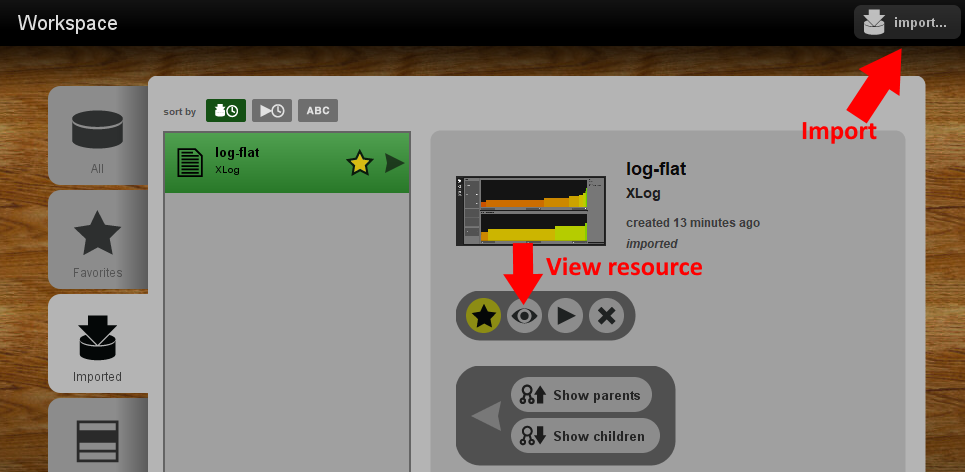
\includegraphics[scale=0.8]{img/ProM_a_overview.png}\\
This results in the following view:\\
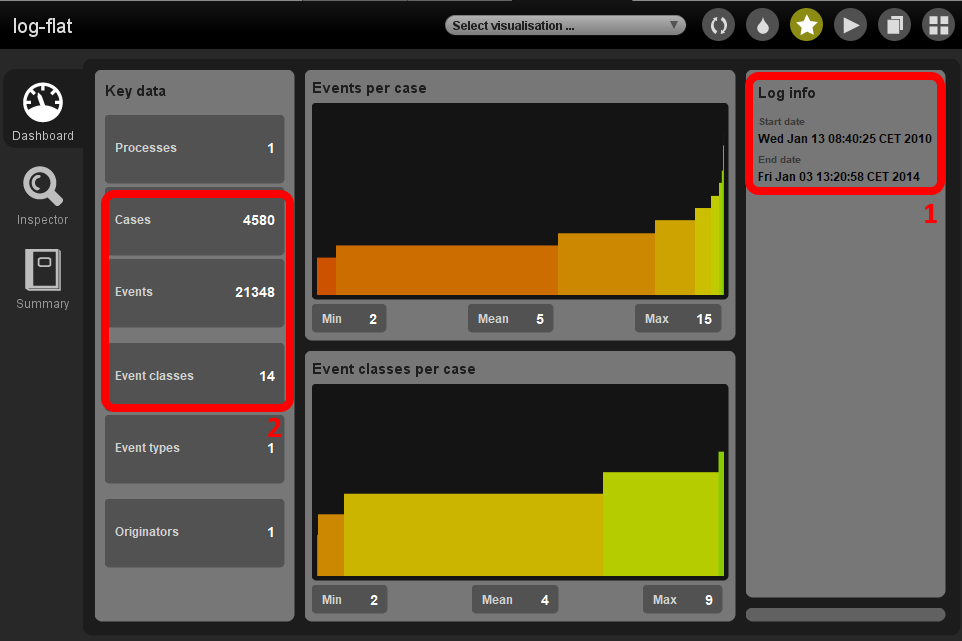
\includegraphics[scale=0.8]{img/ProM_a_overview_2.png}\\
From it we can read 
\begin{itemize}
\item the time period (1) covered by the event log, which is from 13.01.2010 to 03.01.2014
\item the number of cases, events and activities of the log (2), being 4580, 21348 and 14 respectively (note that activities appear in ProM as event classes)
\end{itemize}
To gain more information on the activities we click the summary tab in the left which results in the following view:\\
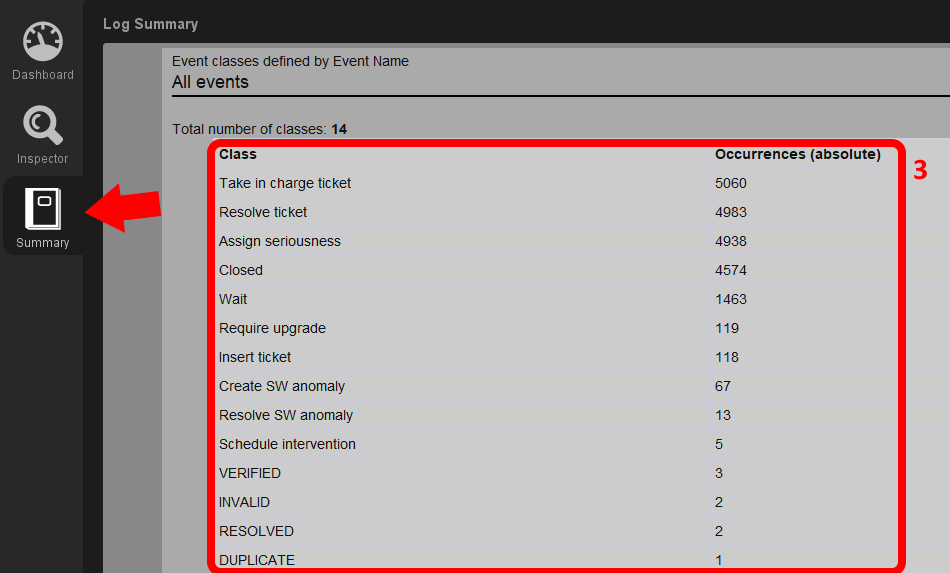
\includegraphics[scale=0.8]{img/ProM_a_summary.png}\\
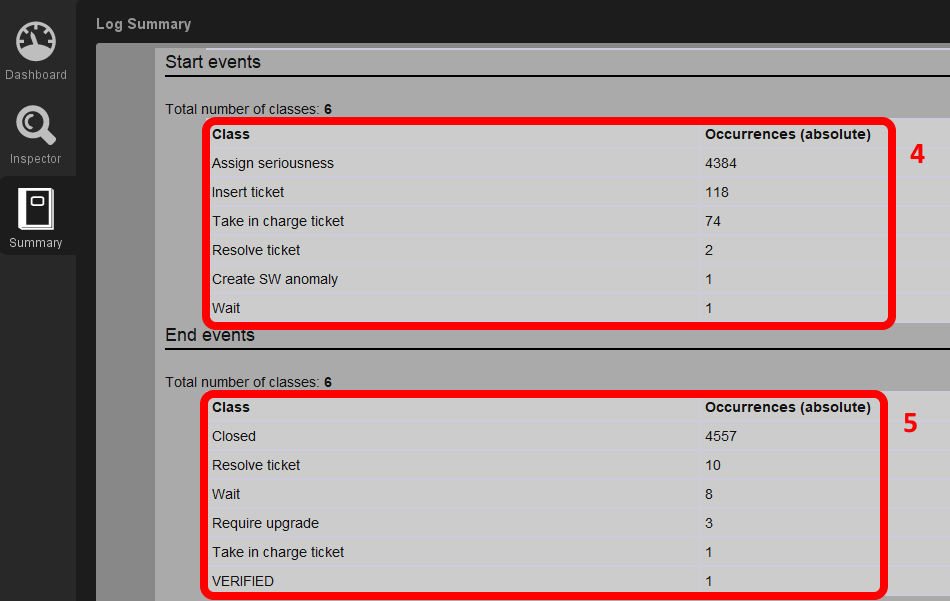
\includegraphics[scale=0.8]{img/ProM_a_summary_2.png}\\
From (3) we get a table of occurence frequencies for each activity. From (4) we get a table of occurence frequencies for each start activity. From (5) we get a table of occurence frequencies for each end activity.



\subsection*{(b)}
\subsection*{(c)}
\subsection*{(d)}

\end{document}